% 第 19 题椭圆坐标图：按固定源 PDF 矢量路径换算（1 pt → 0.03515 cm）。
% 原点取椭圆中心 O（源页 (692.9102, 202.0039) pt，即两轴交点），y 向上。
% 椭圆半轴 56.6719/34.0020（轴比 ≈5:3，源为示意画法），线宽 0.8pt（源为其余图元 2 倍）；
% x 轴左 −76.51 右至箭头 76.51、y 轴下 −56.67 上至箭头 59.51（均穿出椭圆，左右不对称照源）；
% 标签 y/A/x/O 四处；A 标于椭圆上顶点（对应题设 A(0,1)）。无实心点、无刻度。
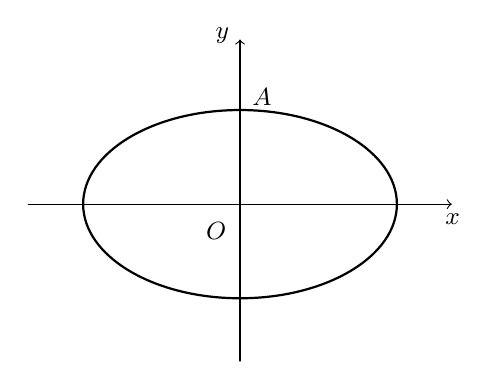
\begin{tikzpicture}[line cap=round,line join=round,font=\small,x=0.03515cm,y=0.03515cm]
% 坐标轴
\draw[->] (-76.51,0)--(76.51,0);
\draw[->] (0,-56.67)--(0,59.51);
% 椭圆（线宽 0.8，与源一致）
\draw[line width=0.8pt] (0,0) ellipse (56.67 and 34.00);
% ===== 标注（照源字形框中心，显式坐标）=====
\node[anchor=center,inner sep=0] at (-6.39,60.94) {\(y\)};
\node[anchor=center,inner sep=0] at (7.91,38.75) {\(A\)};
\node[anchor=center,inner sep=0] at (76.80,-5.57) {\(x\)};
\node[anchor=center,inner sep=0] at (-8.59,-9.66) {\(O\)};
\end{tikzpicture}
